\documentclass{article}

\usepackage{graphicx}
\usepackage{fancyhdr}
\usepackage[sorting=none]{biblatex}
\usepackage[margin=1in]{geometry}
\usepackage{listings}
\usepackage[hidelinks]{hyperref}
\usepackage{xcolor}
\usepackage{xepersian}
\usepackage{ltablex}
\usepackage{booktabs, makecell, longtable}



\addbibresource{bibliography.bib}
\settextfont[Scale=1.2]{IRNazli.ttf}
\setlatintextfont[Scale=1]{times.ttf}
\renewcommand{\baselinestretch}{1.5}
\pagestyle{fancy}
\fancyhf{}
\renewcommand{\headrulewidth}{1pt}
\renewcommand{\footrulewidth}{1pt}
\setcounter{tocdepth}{2}
\begin{document}

\def\by{نگارش}
\def\superv{مدرس}
\def\faculty{دانشکده مهندسی کامپیوتر}
\def\course{رایانش عصبی}
\def\docTitle{پروژه هفتم }
\def\supervisor{دکتر رضا صفابخش}
\def\fname{سیدمهدی }
\def\lname{میرفندرسکی}
\def\stuNum{401131065}
\def\docDate{بهمن 1401}

\rhead{\docTitle}
\lhead{درس \course}
\rfoot{\fname \lname}
\lfoot{\stuNum}
\cfoot{\\ \thepage}



\begin{titlepage}
\begin{center}
%
\includegraphics[width=0.4\textwidth]{fa-logo.png}\\
\centerline{{
\includegraphics[height=3.8cm]{fa-logo}}}        
\LARGE
%\textbf{دانشگاه صنعتی اصفهان}\\
%\textbf{دانشکده مهندسی کامپیوتر}\\
\bf{\fontsize{16pt}{16pt}\selectfont دانشگاه صنعتی امیرکبیر}\par
\fontsize{14pt}{15pt}\selectfont(پلی‌تکنیک تهران)\par
\fontsize{16pt}{17pt}\selectfont \faculty \par
        
\par
        

\vfill
{\huge\settextfont{B_Titr.ttf}{\docTitle  درس  \course}}
\vfill
 
\settextfont[Scale=1.2]{BNazanin.ttf}
{\huge\by}\\
\fontsize{18pt}{19pt}\selectfont\bfseries{\fname \lname} \\
\settextfont[Scale=1.2]{BNazanin.ttf}
{\huge\superv}\\
{\fontsize{18pt}{19pt}\selectfont\bfseries\par\supervisor}\\
\fontsize{16pt}{17pt}\selectfont\docDate\\
 
 
        
\LARGE
%\textbf{نام و نام خانوادگی: مجید فرهادی}\\
%\textbf{شماره دانشجویی: 9700000}\\
%\textbf{نیم‌سال تحصیلی: پاییز 1400}\\
%\textbf{مدرّس: دکتر محمّدرضا حیدرپور}\\
%\textbf{دستیاران آموزشی: مجید فرهادی - دانیال مهرآیین - محمّد نعیمی}\\
\end{center}
\end{titlepage}


\tableofcontents

\newpage



\section{سوالات تشریحی}

\subsection{سوال اول}


برای توضیح نقش نویز در نوع شبکه‌ها فرض می‌کنیم که نویزی برای ورودی به بخش مولد این نوع شبکه‌ها وجود نداشت. اتفاقی که خواهد افتاد این است که قسمت مولد خروجی یکسانی برای تمام برچسب‌ها تولید خواهد کرد. درواقع نویز عامل ایجاد کننده خروجی‌های متفاوت به ازای برچسب‌های یکسان خواهد بود.  به بیان دیگر این نویز به عنوان منبع تغییرات در نمونه‌های تولید شده عمل می‌کند. با اضافه‌کردن نویز، مولد می‌تواند طیف متنوعی از نمونه‌ها را تولید کند که باعث می‌شود روند آموزش قوی‌تر و مقاوم‌تر شود. همچنین اضافه کردن نویز از \lr{mode collapse} جلوگیری خواهد کرد که در سوال بعد به آن پرداخته شده است.

تغییر پارامتر یا توزیع نویز به مولد در این نوع شبکه‌ها می‌تواند تأثیر قابل توجهی بر کیفیت و تنوع نمونه‌های تولید شده و همچنین بر پایداری فرآیند آموزش بگذارد. هرچه نویز بسته به پارامتر و توزیع تصادفی‌تر باشند، می‌تواند منجر به تنوع بیشتر در نمونه‌های تولید شده شود. زیرا مولد تشویق می‌شود تا مناطق مختلف فضای ورودی را کاوش کند. و این اتفاق، جلوگیری از \lr{mode collapse} در فضای ورودی را به دنبال دارد. با این حال، تصادفی‌تر بودن نویز می‌تواند یادگیری ساختار داده‌ها را برای مولد دشوارتر کند و در نتیجه نمونه‌های با کیفیت پایین‌تری تولید شوند. درواقع پیداکردن پارامتر و توزیع مناسب نویز یک نوع trade-off میان تشویق مولد برای کاوش در فضای ورودی و یادگیری ساختار داده‌ها در مولد خواهد بود. 


% -------------------------------------------------------------------
\subsection{سوال دوم}

این دو نوع مسئله دو مشکل رایجی هستند که می‌توانند هنگام آموزش شبکه‌های مولد تقابلی رخ دهند.

\lr{mode collapse} مشکلی است که در آن مولد به جای تولید طیف متنوعی از نمونه‌ها، تغییرات محدودی از یک نمونه تولید می‌کند. این زمانی اتفاق خواهد افتاد که مولد در فریب دادن تمایزگر بیش از حد خوب شود و گرادیان‌ها از تمایزگر به مولد بسیار کوچک شود و باعث شود که مولد در فضای ورودی به یک نقطه (زیرمجموعه ای از داده‌های آموزشی) همگرا شود. سپس باعث می‌شود که مولد قادر به تولید نمونه‌های جدید و متفاوت از داده‌های آموزشی نباشد.

\lr{diminishing gradients} مشکل دیگری است که می‌تواند در طول آموزش رخ دهد. این مشکل زمانی اتفاق می‌افتد که گرادیان‌ها از تمایزگر به مولد بسیار کوچک شده و باعث می‌شوند که مولد به کمینه محلی همگرا شود. این مشکل ناشی از رسیدن مولد و تمایزگر به تعادلی است که در آن مولد قادر به تولید نمونه‎هایی است که از نمونه‌های واقعی قابل تشخیص نیستند، اما گرادیان‌های تشخیص دهنده برای ادامه بهبود مولد بسیار کوچک خواهد بود.

برای جلوگیری از این مشکلات، چندین تکنیک وجود دارد که می‌توان از آنها استفاده کرد:
\begin{itemize}
    \item منظم‌سازی: تکنیک‌هایی مانند \lr{Drop out} و کاهش وزن را می‌توان برای جلوگیری از بیش‎برازش مولد و تمایزگر به داده‌های آموزشی استفاده کرد.
    \item هموارسازی یک طرفه برچسب‌ها: اگر خروجی تمایزگر را برای اطمینان کمتر در پیش بینی‌های خود به صورت مقدار پیوسته‌ای بین 0 و 1 به‌جای خود اعداد 0 و 1 انتخاب کنیم، می‌توانیم به بهبود گرادیان‌ها از تمایزگر به مولد کمک کند
    \item استفاده از نویز: افزودن نویز تصادفی‌تر به ورودی مولد می‌تواند با تشویق مولد به کاوش در مناطق مختلف فضای ورودی به جلوگیری از \lr{mode collapse} کمک کند.
    \item برنامه آموزشی: استفاده از یک زمانبندی آموزشی برای تمایزگر و مولد به صورت متناوب با افزایش دوره‌ای نرخ یادگیری به جلوگیری از \lr{diminishing gradients} کمک می‌کند.
    \item تغییرات معماری: استفاده از معماری‌هایی که بهینه‌سازی مولد و تمایزگر را سخت‌تر (استفاده از لایه‌های عادی) می‌کند، می‌تواند به بهبود پایداری فرآیند آموزش کمک کند.
\end{itemize}

ترکیبی از این تکنیک‎ها می‌تواند برای بهبود عملکرد این نوع شبکه‌ها مورد استفاده قرار گیرد. 
% -------------------------------------------------------------------
\subsection{سوال سوم}
لایه معکوس کانولوشن عملکردی مخالف لایه کانولوشنی دارد. به بیان دیگر با ورود یک \lr{feature map} به این نوع لایه، یک تصویر ساخته می‌شود. می‌توان گفت لایه معلکوس کانوولوشنی اطلاعات خلاصه شده چند پیکسل (خلاصه شده توسط لایه کانوولوشنی) را توسعه و بسط می‌دهد. این نوع لایه‌ها با استفاده از فرمولی برای تابع گسترش نقطه، تخمین بهبود یافته‌ای از تصویر ایجاد ارائه می‌کنند.

 معماری یک \lr{DCGAN} از دو جزء اصلی مولد و تمایزگر تشکیل می‌شود. شبکه مولد یک بردار نویز تصادفی را به عنوان ورودی می‌گیرد و با عبور دادن آن از یک سری لایه معکوس کانولوشن، که برای افزایش وضوح فضایی ورودی طراحی شده‌اند، تصویر جدیدی تولید می‌کند. خروجی مولد یک تصویر مصنوعی است که از یک تصویر واقعی قابل تشخیص نیست. شبکه تمایزگر هم تصاویر واقعی و هم تصاویر مصنوعی تولید شده توسط مولد را به عنوان ورودی می‌گیرد. سپس از یک سری لایه‌های کانولوشنی برای تعیین واقعی یا مصنوعی بودن هر تصویر استفاده می‌کند. خروجی تمایزگر یک مقدار اسکالر بین 0 و 1 است که 0 نشان دهنده یک تصویر مصنوعی و 1 نشان‌دهنده یک تصویر واقعی است. این دو شبکه با هم در یک فرآیند رقابتی آموزش می‌بینند، به طوری که مولد سعی می‌کند تصاویری را تولید کند که تمایزگر آنها را به عنوان واقعی طبقه بندی کند، و تمایزگر سعی می‌کند به درستی تصاویر تولید شده را به عنوان مصنوعی طبقه بندی کند. با پیشرفت آموزش، تولید کننده در تولید تصاویر واقعی بهتر می‌شود و تمایزگر در شناسایی تصاویر مصنوعی بهتر می شود.


ایده اصلی تولید تصویر از متن این است که مولد و تمایزگر را در یک \lr{GAN} با کدگذاری متنی مناسب توضیحات تقویت کنیم. از نظر مفهومی، این شبیه به شرطی کردن عملکرد مولد و تمایزگرها بر روی توضیحات متن است. کار اصلی پیاده‌سازی را با استفاده از شبکه‌های عصبی کانولوشنی عمیق توصیف می‌کند و از این رو \lr{DCGAN} نامیده می‌شود. مولد یک شبکه لایه‌های معکوس کانولوشنی است که تصویری را از متن بر اساس توزیع نویز تولید می‌کند. تمایزگر یک شبکه کانولوشنی است که با توجه به کدگذاری متن، احتمال تعلق تصویر ورودی به توزیع داده اصلی را خروجی می‌دهد. البته جزئیات معماری در لینک موجود است (تعداد لایه‌ها، توابع فعالیت و ...). اما نکته بدیهی که لازم به ذکر است که آموزش تمایزگر بر اساس کپشن تصاویر اتفاق خواهد افتاد. یعنی باید داده‌های آموزشی با متن موجود باشند.


% -------------------------------------------------------------------
\subsection{سوال چهارم}
شبکه‌های مولد تقابلی از دو جزء اصلی تشکیل شده‌اند: یک شبکه مولد و یک شبکه تمایزکر. روند آموزش این دو شبکه متفاوت و مکمل یکدیگر است. معماری این نوع شبکه‌ها در شکل زیر آورده شده است.

\begin{figure}[!h]
    \centering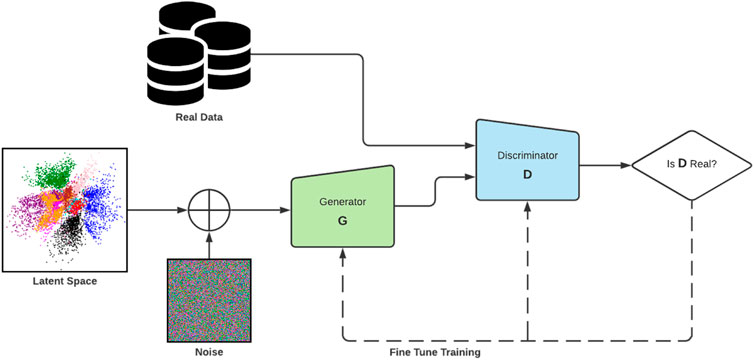
\includegraphics[scale=.55]{./p4}
    \caption{معماری شبکه‌های مولد تقابلی}\label{fig.41}
\end{figure}

همانطور که در شکل مشاهده می‌شود، شبکه مولد برای تولید نمونه‌های جدید که مشابه داده‌های آموزشی هستند آموزش داده می‌شود. این کار با به حداقل رساندن تفاوت بین نمونه‌های تولید شده و نمونه‌های واقعی انجام می‌شود (با استفاده از یک الگوریتم بهینه‌سازی مانند \lr{GD} برای به حداقل رساندن یک تابع هزینه). تابع هزینه مورد استفاده در \lr{GAN} معمولاً \lr{cross-entropy} خواهد بود.

از طرفی شبکه تمایزگر برای تشخیص تمایز بین نمونه‌های واقعی و تولیدشده آموزش داده می‌شود. این کار با به حداکثر رساندن تفاوت بین احتمال یک نمونه واقعی و احتمال یک نمونه تولیدشده جدید انجام می‌شود. هر دو شبکه به طور همزمان آموزش می‌بینند، به طوری که مولد در تلاش برای تولید نمونه‌هایی است که می‌تواند تمایزگر را فریب دهد و تمایزگر تلاش می‌کند تا نمونه‌های تولید شده را به درستی شناسایی کند. به خاطر همین فرایند یک فرایند رقابتی خواهد بود.

تابع خطا در مدل \lr{GAN} بدین صورت تعریف می‌شود که هر چه تصاویر تولید شده توسط مولد واقعی‌تر باشد و تمایزگر را به خطا بیاندازد به مولد هزینه کمتری داده میشود و هرچه تمایزگر بهتر بتواند تصاویر را تشخیص دهد هزینه کمتری برای آن در نظر گرفته می‌شود. تابع هزینه به شرح زیر است:
$$
\min_{G}\max_{D}\mathbb{E}_{x\sim p_{\text{data}}(x)}[\log{D(x)}] +  \mathbb{E}_{z\sim p_{\text{z}}(z)}[1 - \log{D(G(z))}]
$$

% -------------------------------------------------------------------

\section{\lr{CGAN}}
\subsection{سوال اول}

در \lr{CGAN}، برای ادغام یک برچسب در یک تصویر، باید هم برچسب و هم یک بردار نویز را به عنوان ورودی به مولد ارسال کرد. سپس مولد از این اطلاعات برای تولید تصویری که بر روی برچسب شرطی شده است استفاده می‌کند. برچسب را می‌توان قبل از ارسال آن به مولد به بردار نویز متصل کرد یا می‌توان آن را به عنوان ورودی جداگانه به مولد ارسال کرد. سپس مولد از اطلاعات برچسب برای کنترل ویژگی‌های تصویر تولید شده استفاده می‌کند. از طرفی در تمایزگر نیز به همین دو روش می‌توان برای آموزش برچسب را با ورودی ادغام کرد.


% -------------------------------------------------------------------
\subsection{سوال دوم}

در یک \lr{GAN} استاندارد، تمایزگر معمولاً یک مقدار اسکالر واحد را خروجی می‌دهد که احتمال اینکه ورودی یک نمونه واقعی (تولید نشده) باشد را نشان می‌دهد. در یک \lr{CGAN}، تمایزگر یک مقدار اسکالر واحد را نیز خروجی می‌دهد که احتمال اینکه ورودی یک نمونه واقعی باشد را نشان می‌دهد. با این حال، در یک \lr{CGAN}، تمایزگر همچنین یک برچسب یا سایر اطلاعات شرطی را به عنوان ورودی می‌گیرد و از این اطلاعات برای طبقه‌بندی خود استفاده می‌کند. بنابراین، خروجی تمایزگر در \lr{CGAN} یک مقدار اسکالر است که نشان دهنده احتمال این است که ورودی چقدر واقعی است، پس برچسب ورودی در آن جایی نخواهد داشت.
% -------------------------------------------------------------------


\subsection{سوال سوم}

ابتدا لازم به ذکر است که، برای پیاده‌‌سازی این قسمت، با توجه به سوال نیاز به سعی و خطا نبود و چند مقاله پیاده‌سازی شده بررسی شد. راه‌های مختلفی برای این مسئله پیشنهاد شده‌اند (استفاده از لایه کانولوشنی و یا لایه Dense ساده). با پیاده‌سازی فعلی بر اساس لایه‌های Dense ساده نتیجه مطلوبی گرفته شد. 

روال کار بدین صورت است که ابتدا تنها داده‌ها (بدون برچسب) را به بازه -1 و 1 انتقال می‌دهیم (تقسیم بر 255، منهای 1 و ضربدر 2). سپس سه مرحله اساسی ساخت مدل‌های تمایزگر، مولد و آموزش ترکیبی این دو را خواهیم داشت، که در ادامه اقدام به توضیح هر یک می‌پردازیم:

\begin{itemize}
    \item مدل تمایزگر یک تصویر به همراه برچسب آن از مجموعه داده می‌گیرد و تشخیص می‌دهد که آیا یک تصویر واقعی یا ساختگی است. اما برای ورودی مدل باید ابتدا بتوان آن‌ها را به نحوی ترکیب کرده و به مدل دهیم. ابتدا برچسب کلاس از یک لایه Embedding با خروجی 784 عبور داده می‌شود (با اندازه حداکثر 10). این کار به دلیل آن است که برای ادغام با تصاویر در نهایت در با تصاویر ضرب خواهند شد. سپس سه لایه Dense قرار می‌گیرد. برای هر لایه نیز مانند اکثر پیاده‌سازی‌ها از تابع فعالیت LeakyReLU استفاده شد. درنهایت برای تولید مقدار احتمال بین 0 و 1 برای واقعی یا جعلی بودن تصاویر از یک نورون به همراه تابع فعالیت sigmoid استفاده شد.
    \item مدل مولد یک مقدار از فضای پنهان (latent space) را به عنوان ورودی می‌گیرد و یک تصویر را خروجی می‌دهد. مشابه مدل تمایزگر این فضای پنهان با برچسب تصویر خواسته شده ادغام می‌شود. روال کار به همان صورت خواهد بود. اما بعد از ادغام فضای پنهان (معمولا اندازه آن را 100 درنظر می‌گیرند) یک فضای برداری از مقادیر تصادفی (توزیع گاوسی) تشکیل شده است که با برچسب نیز در آن نهفته شده است. درنهایت پس از آماده‌سازی ورودی سه لایه Dense قرار گرفته‌اند که بعد از هر سه لایه یک لایه BatchNormalization با تکانه 0.8 قرار گرفته است. این کار برای آموزش بهتر شبکه انجام می‌شود (بدون لایه‌های ذکر شده تست شد و نتیجه خوبی گرفته نشد.). درنهایت نیز برای خروجی یک لایه به اندازه 784 در نظر گرفته شد. 
    \item یک مدل نهایی می‌تواند یک مدل مولد با ورودی‌های مدل تمایزگر و داده‌های آموزشی به همراه برچسب است. برای ساخت این مدل ابتدا مدل فوق را ساخته و به صورت نوبتی تمایزگر و مولد را آموزش می‌دهیم. برای اینکار به صورت دستی ای‌پاک‌ها و دسته‌ها را پیاده‌سازی می‌کنیم. همچنین باید در هر حلقه ابتدا تمایزگر را یکبار برای داده‌های آموزشی و یکبار برای داده‌های جعلی آموزش داده و سپس وزن‌های آن را ثابت نگه داریم و آموزش مولد را شروع کنیم. همچنین برای بهبود آموزش از تکنیک هموارسازی برچسب‌‌ها (سوال 2) با پارامتر 0.1 استفاده شد. با توجه به ساختار درنظر گرفته شده نمودار خطای هریک (مولد و تمایزگر) در ادامه مشخص شده است (نمودار خطای کل مدل همان خطای مولد درنظر گرفته شده است.). آموزش با 20 ای‌پاک انجام شد که تصاویر آن به همراه gif مربوطه ضمیمه شده است. 
\end{itemize}

\begin{figure}[!h]
    \centering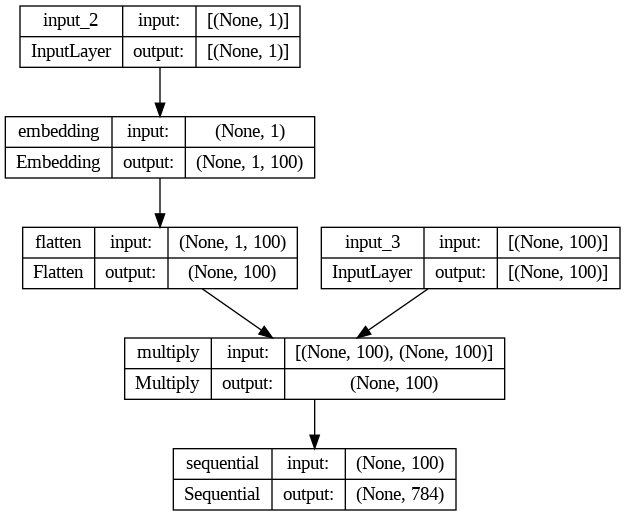
\includegraphics[scale=.55]{./gen-1}
    \caption{گراف مصور مولد}\label{fig.31}
\end{figure}

\begin{figure}[!h]
    \centering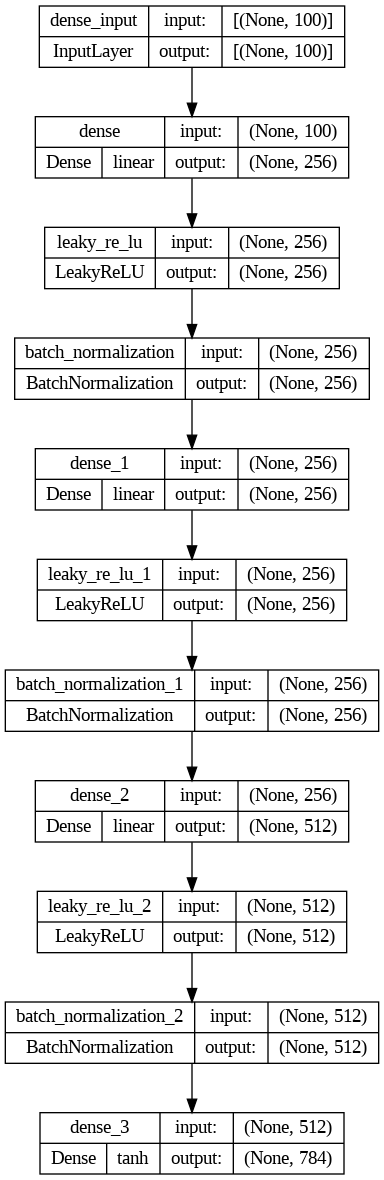
\includegraphics[scale=.55]{./gen-2}
    \caption{گراف مصور مولد}\label{fig.32}
\end{figure}

\begin{figure}[!h]
    \centering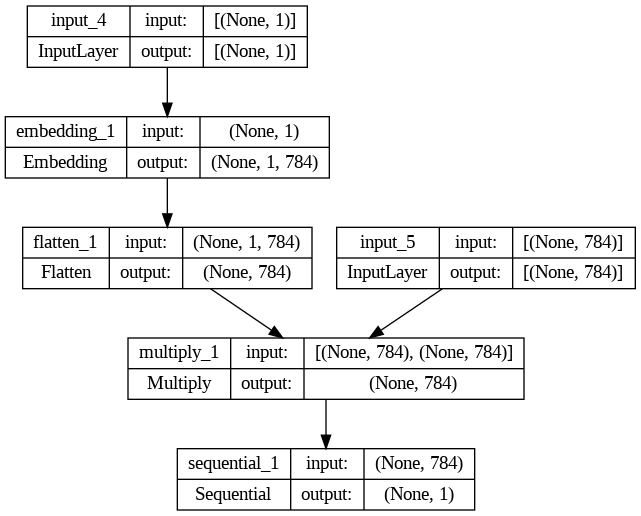
\includegraphics[scale=.55]{./dis-1}
    \caption{گراف مصور تمایزکر}\label{fig.33}
\end{figure}

\begin{figure}[!h]
    \centering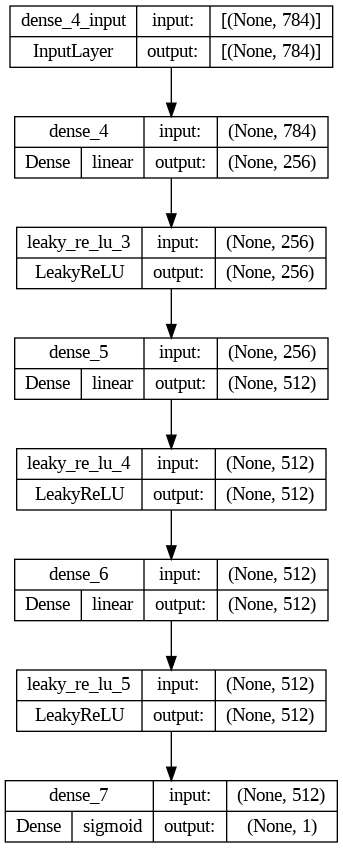
\includegraphics[scale=.55]{./dis-2}
    \caption{گراف مصور تمایزکر}\label{fig.34}
\end{figure}

\begin{figure}[!h]
    \centering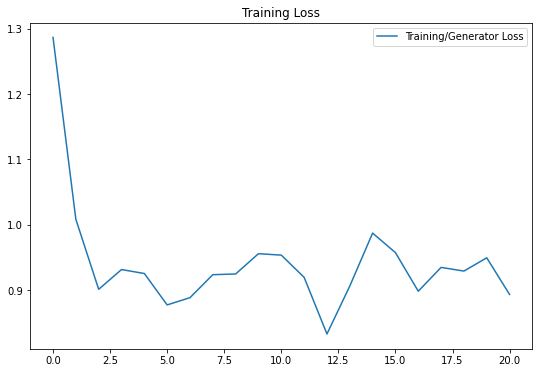
\includegraphics[scale=.55]{./loss-1}
    \caption{نمودار خطا}\label{fig.35}
\end{figure}

\begin{figure}[!h]
    \centering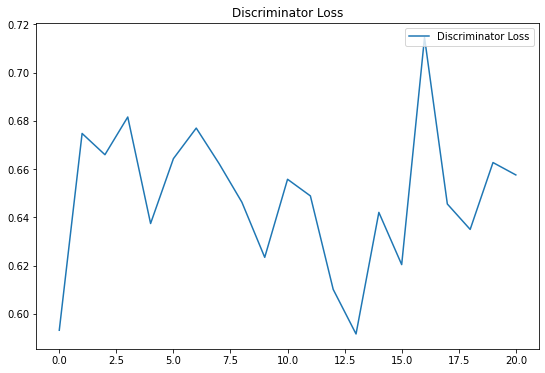
\includegraphics[scale=.55]{./loss-2}
    \caption{نمودار خطا}\label{fig.36}
\end{figure}

همانطور که در نمودار خطای آموزش مشاهده می‌شود، مدل پس از چند ای‌پاک به یک محدوده‌ای همگرا می‌شود. در واقع در این محدوده به طور پیوسته مولد و تمایزگر دچار نوسان یا همان رقابت هستند تا بر دیگری غالب شوند. این یکی از معماری از یکی از پیاده‌سازی‌های موجود الهام گرفته است. برای دستیابی به خطای کمتر باید معماری یا تکنیک‌های دیگری بکار برد.

% \section{سوال اول}
% اساسا با این کار به نوعی می‌توانیم داده‌های سری زمانی را به یک مسئله یادگیری نظارت‌شده یا بدون نظارت تبدیل کنیم. در واقع در نظر گرفتن لگ‌ها در تجزیه و تحلیل سری‌های زمانی بسیار مفید هستند زیرا در بین داده‌های سری زمانی خودهمبستگی وجود دارد که همبستگی مقادیر درون یک سری زمانی با مقادیر قبلی خود است. البته بسته به مسئله هرچه از داده فعلی دور شویم، امکان دارد این همبستگی کم یا زیاد شود. با این کار در این مسئله، مشخص می‌کنیم که شبکه نسبت به چقدر داده‌های قبلی حساس باشد. به عنوان مثال احتمالا در مسئله بورس بیشتر از شش ماه گذشته وابستگی نخواهند داشت.

% در ادامه برای حل این بخش تعداد گام‌های ورودی برابر با 32 و همچنین با \lr{offset} یک، پنجره‌ها ایجاد شدند. عدد 32 بدین دلیل بود که تاریخچه نزدیک به یک ماه درنظر گرفته شود.

% % -------------------------------------------------------------------

% \section{سوال دوم}
% برای آموزش شبکه تلاش‌های بسیاری صورت گرفت اما نتایج قابل قبولی دریافت نشد. درنهایت معماری انتخاب شده بدین صورت است که یک لایه \lr{SimpleRNN}، یک لایه \lr{Dense} و در نهایت یک تک نورون برای مسئله دسته‌بندی در نظر گرفته شد. درضمن تابع فعالیت خروجی شبکه‌ها سیگموید و توابع فعلیت لایه‌های دیگر \lr{relu} درنظر گرفته شد. همچنین سایز دسته برابر 16 و ای‌پاک برابر با 10 درنظر گرفته شد. مشابه تمرینات قبل کالبک زیر نیز گذاشته شد.

% \lr{es-callback = EarlyStopping(monitor="val-loss", patience=3, restore-best-weights=True)}

% در جدول زیر ترکیبات مختلف تعداد واحدها مشاهده می‌شود.

% \begin{table}[!h]
%     \centering
%     \begin{tabular}{|c|c|c|c|c|c|}
%     \hline
%     شماره & \lr{SimpleRNN} & \lr{Dense} & آموزشی صحت & اعتبارسنجی صحت & تست صحت \\ \hline
%     1 & 1 & 16 & $58.57$ & $58.17$ & $58.03$ \\ \hline
%     2 & 2 & 16 & $58.57$ & $58.17$ & $58.03$ \\ \hline
%     3 & 3 & 16 & $58.57$ & $58.17$ & $58.03$ \\ \hline
%     4 & 4 & 16 & $56.52$ & $62.5$ & $57.79$ \\ \hline
%     5 & 5 & 16 & $59.05$ & $59.13$ & $57.79$ \\ \hline
%     6 & 6 & 16 & $58.57$ & $58.17$ & $58.03$ \\ \hline
%     7 & 7 & 16 & $59.12$ & $58.65$ & $57.55$ \\ \hline
%     8 & 1 & 32 & $58.57$ & $58.17$ & $58.03$ \\ \hline
%     9 & 2 & 32 & $58.78$ & $58.65$ & $57.55$ \\ \hline
%     10 & 3 & 32 & $58.85$ & $58.65$ & $58.03$ \\ \hline
%     11 & 4 & 32 & $58.57$ & $58.17$ & $58.03$ \\ \hline
%     12 & 5 & 32 & $59.05$ & $61.54$ & $61.15$ \\ \hline
%     13 & 6 & 32 & $58.57$ & $58.17$ & $58.03$ \\ \hline
%     14 & 7 & 32 & $58.57$ & $58.17$ & $58.03$ \\ \hline
%     15 & 1 & 64 & $58.57$ & $58.17$ & $58.03$ \\ \hline
%     16 & 2 & 64 & $58.5$ & $62.02$ & $59.71$ \\ \hline
%     17 & 3 & 64 & $58.64$ & $58.65$ & $57.79$ \\ \hline
%     18 & 4 & 64 & $58.85$ & $58.65$ & $57.55$ \\ \hline
%     19 & 5 & 64 & $58.57$ & $58.17$ & $58.03$ \\ \hline
%     20 & 6 & 64 & $58.98$ & $57.69$ & $58.99$ \\ \hline
%     21 & 7 & 64 & $60.29$ & $60.1$ & $59.23$ \\ \hline
%     22 & 1 & 128 & $58.57$ & $58.17$ & $58.03$ \\ \hline
%     23 & 2 & 128 & $58.57$ & $58.17$ & $58.03$ \\ \hline
%     24 & 3 & 128 & $58.57$ & $58.17$ & $58.03$ \\ \hline
%     25 & 4 & 128 & $58.23$ & $60.1$ & $60.43$ \\ \hline
%     26 & 5 & 128 & $57.89$ & $60.58$ & $60.19$ \\ \hline
%     27 & 6 & 128 & $58.5$ & $61.54$ & $61.15$ \\ \hline
%     28 & 7 & 128 & $57.61$ & $62.5$ & $58.03$ \\ \hline



% \end{tabular}
% \end{table}


% \cleardoublepage

% با در نظر گرفتن صحت محموعه آموزشی و اعتبارسنجی معماری زیر انتخاب شد:

% \begin{table}[!h]
%     \centering
%     \begin{tabular}{|c|c|c|c|c|c|}
%     \hline
%     شماره & \lr{SimpleRNN} & \lr{Dense} & آموزشی صحت & اعتبارسنجی صحت & تست صحت \\ \hline
%     16 & 2 & 64 & $58.5$ & $62.02$ & $59.71$ \\ \hline

% \end{tabular}
% \end{table}


% همچنین نمودار صحت و خطای مجموعه آموزشی و اعتبارسنجی برای بهترین معماری در ادامه مشاهده می‌شود.

% \begin{figure}[!h]
%     \centering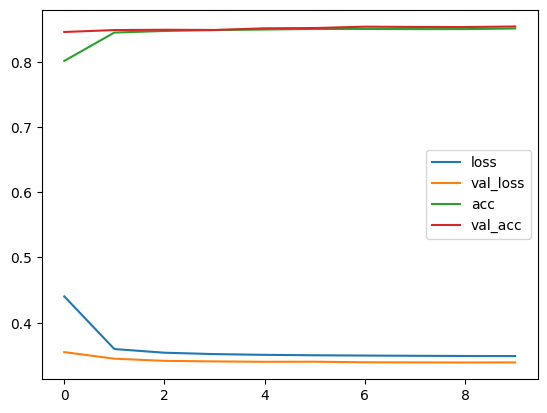
\includegraphics[scale=.40]{./p2-1}
%     \caption{نمودار صحت و خطای بهترین معماری}\label{fig.21}
% \end{figure}

% \cleardoublepage

% % -------------------------------------------------------------------

% \section{سوال سوم}
% برای این بخش یک مدل شبکه کانولوشنی آموزش دیده شد. توجه شود که برای این قسمت سعی و خطا در نظر گرفته نشده است (سعی و خطا شبکه کانولوشنی در پروژه چهارم). معماری شبکه طراحی شده و نتایج آن در ادامه مشاهده می‌شود.

% \begin{figure}[!h]
%     \centering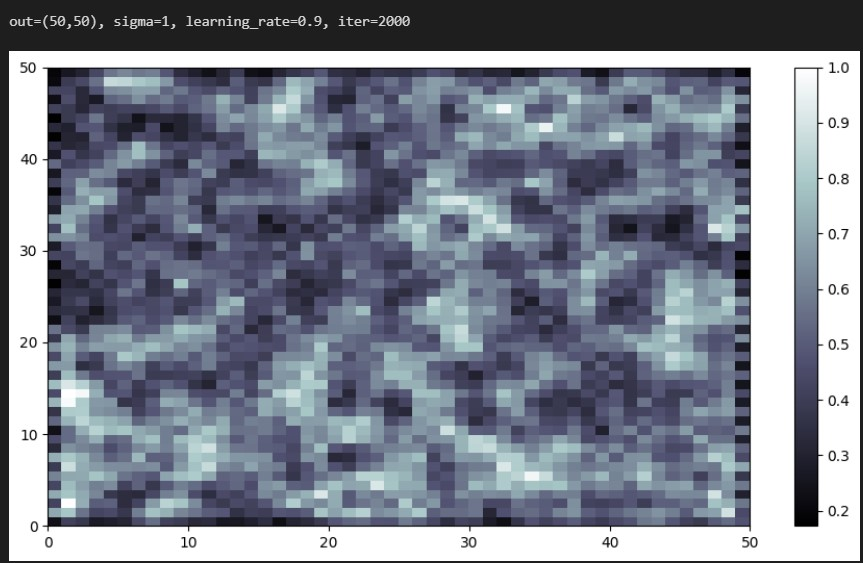
\includegraphics[scale=.55]{./p3-1}
%     \caption{معماری شبکه کانولوشنی}\label{fig.31}
% \end{figure}

% \begin{figure}[!h]
%     \centering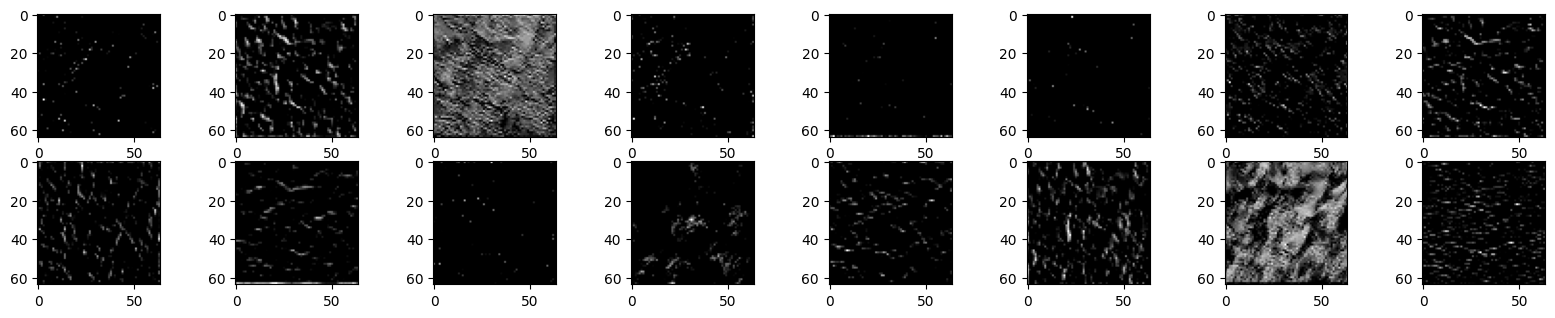
\includegraphics[scale=.40]{./p3-2}
%     \caption{نمودارهای شبکه کانولوشنی}\label{fig.32}
% \end{figure}

% \cleardoublepage

% همانطور که مشاهده می‌شود این شبکه کانولوشنی تقریبا در حد بهترین شبکه قسمت قبل عمل کرده است (می‌توان گفت کانولوشنی حتی مقداری بهتر عمل کرده است.) . همچنین احتمالا با سعی و خطا بتوان نتایج بهتری را نیز کسب کرد. پس در کل اینگونه برداشت شد که شبکه کانولوشنی برای این مسئله بهتر عمل می‌کند.

% % -------------------------------------------------------------------

% \section{سوال چهارم}
% در این گزارش ابتدا انواع ناهنجاری‌ها بیان شده است: (داده‌های پرت افزایشی، تغییرات زمانی و تغییر سطح یک پدیده). در ادامه مجموعه داده قیمت بیتکوین برای ادامه کار درنظر گرفته شده است. سپس مجموعه آموزشی و تست را ایجاد و آن‌ها را با یک روش یکسان نرمالایز کرده است. در نهایت برای آخرین قسمت پیش‌پردازش مقدار لگ 30 برای آموزش انتخاب شده است. سپس شبکه خود کدگذاری با معماری زیر شامل لایه کانولوشنی و \lr{LSTM} طراحی کرده است. سپس به آموزش شبکه پرداخته شد (بوضوح ورودی و خروجی شبکه داده‌های آموزشی هستند). سپس مشابه تمارین گذاشته با نمودارهای خطای آموزش و اعتبارسنجی، بایاس و واریانس مدل را بررسی می‌کند. حال که مدل از نظر بایاس و واریانس مطلوب است، نوبت به محاسبه خطای بازسازی کل شبکه خود کدگذار می‌رسد. در این مرحله خطای بازسازی داده‌های آموزشی و تست محاسبه می‌شوند. در داده‌های تست اگر مقداری از حداکثر مقدار خطای آموزشی (\lr{mae}) بیشتر باشد، در لیست ناهنجاری‌ها ذخیره می‌شود (اساس این روش بر این اساس است که اگر داده‌ای از تست بازسازی مناسبی نداشت به عنوان ناهنجاری شناخته شود.).

% \begin{figure}[!h]
%     \centering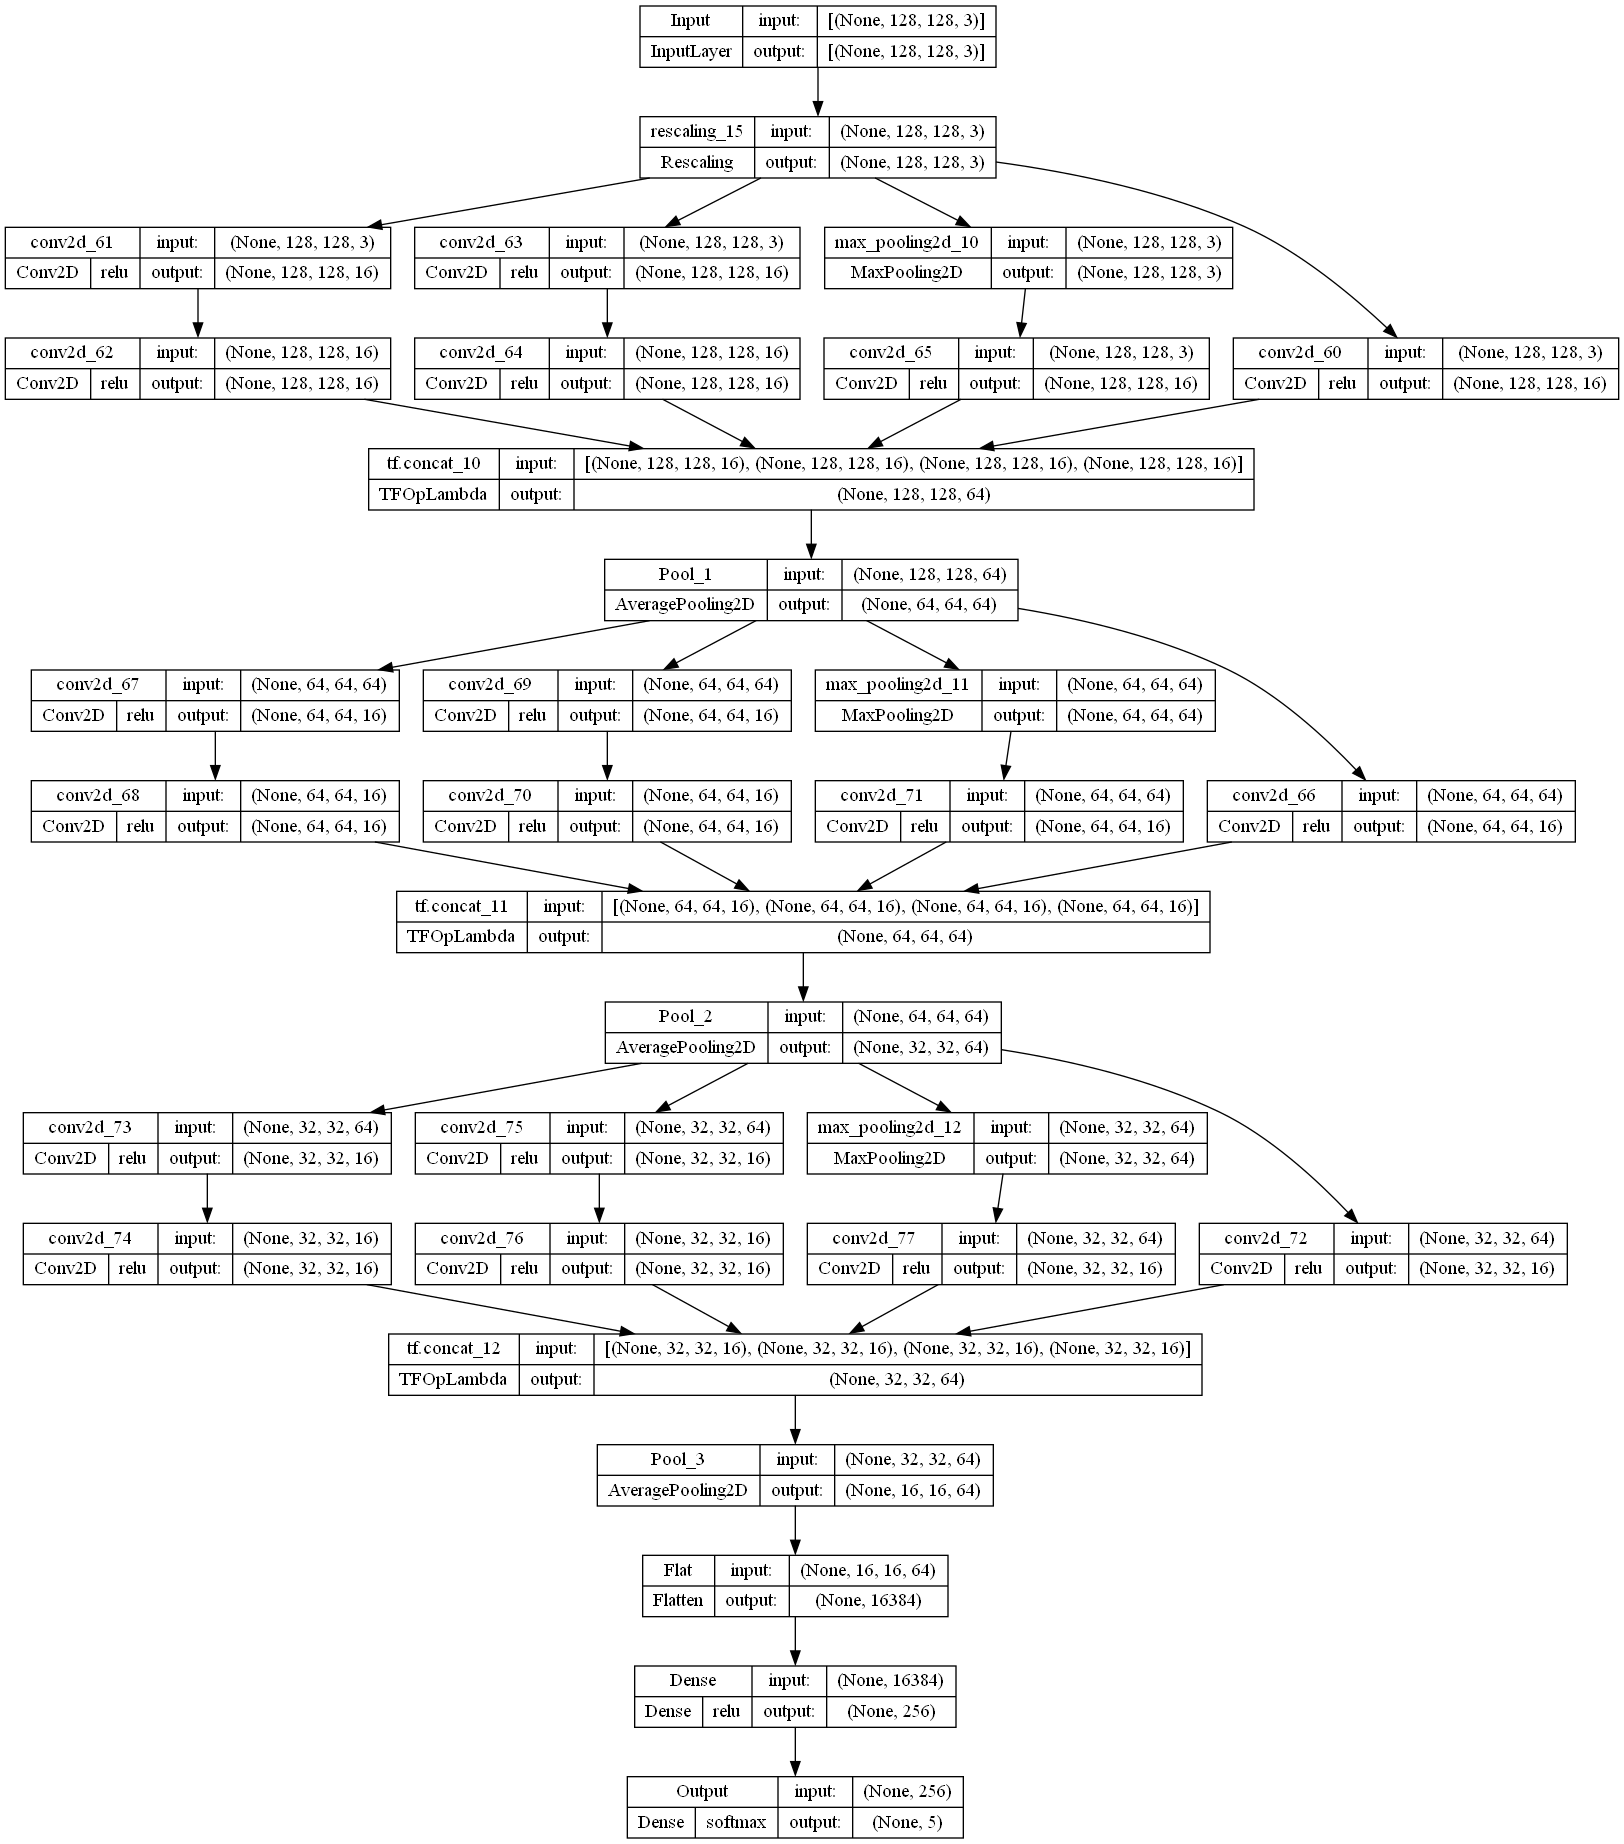
\includegraphics[scale=.55]{./p4-1}
%     \caption{معماری سوال چهارم}\label{fig.41}
% \end{figure}
% % -------------------------------------------------------------------

% \section{سوال پنجم}
% این مقاله از شبکه‌های خود کدگذار برای یادگیری خود نظارتی در مسائل بینایی ماشین استفاده کرده است. بدین صورت که ابتدا یک شبکه‌ خود کدگذار نامتقارن با قسمت کدگذار با پارمترهای بیشتر در نظر گرفته است. سپس به صورت تصادفی بعضی پیکسل‌های ورودی را ماسک (صفر) کرده است. البته کار متمایزی که این مقاله انجام داده است این است که حدود 75 درصد ورودی را ماسک کرده است و 25 درصد باقی مانده را جهت آموزش به شبکه خودکدگذار وارد کرده است. که همین امر باعث افزایش سرعت شده است. و درنهایت وقتی آموزش شبکه به اتمام رسید. ماسک‌های تصاویر تنها به قسمت کدگشای شبکه داده می‌شود تا تصویر بازسازی شود. این ایده کمک بسیار زیادی به تکمیل تصاویر ناقص می‌کند. نکته قابل توجه این خواهد بو.د که داده‌های ماسک شده امکان ورود به کدگذار را نخواهند داشت و تنها باید به قسمت کدگشا وارد شود.

% -------------------------------------------------------------------

\end{document}